\documentclass{experimentreport}

\usepackage{listings}
\usepackage{xcolor}

\definecolor{codegreen}{rgb}{0,0.6,0}
\definecolor{codegray}{rgb}{0.5,0.5,0.5}
\definecolor{codepurple}{rgb}{0.58,0,0.82}
\definecolor{backcolour}{rgb}{0.95,0.95,0.92}
\definecolor{lightgreen}{rgb}{0,0.4,0}
\definecolor{lightred}{rgb}{0.4,0,0}

\definecolor{mygray}{gray}{.9}

% \lstdefinestyle{mystyle}{
\lstset{
    %backgroundcolor=\color{backcolour},   
    commentstyle=\color{brown},
    keywordstyle=\color{magenta},
    numberstyle=\tiny\color{codegray},
    stringstyle=\color{codepurple},
    basicstyle=\ttfamily\tiny,
    breakatwhitespace=false,         
    breaklines=true,                 
    captionpos=b,                    
    keepspaces=true,                 
    numbers=none,                    
    numbersep=5pt,                  
    showspaces=false,                
    showstringspaces=false,
    showtabs=false,                  
    tabsize=2,
    escapeinside={<@}{@>}
}

% \lstset{
% basicstyle=\ttfamily\bfseries\footnotesize,
%   morekeywords={virtualinvoke},
%   keywordstyle=,
%   ndkeywordstyle=\color{red},
%   commentstyle=\color{gray},
%   stringstyle=\color{green},
%   numbers=none,
%   breaklines=true,
%   numberstyle=\ttfamily\footnotesize\color{gray},
%   stepnumber=1,
%   numbersep=6pt,
%   backgroundcolor=\color{white},
%   tabsize=4,
%   showspaces=false,
%   showstringspaces=false,
%   xleftmargin=6pt,
%   captionpos=t
% }

\lstdefinelanguage{JavaScript}{
  keywords={typeof, new, true, false, catch, function, return, null, catch, switch, var, if, in, while, do, else, case, break, export, static, const, let, class, void, async, await, interface, extends, public, this},
  % basicstyle=\linespread{1.0}\ttfamily\footnotesize,
  % keywordstyle= \color{violet}\bfseries,
  ndkeywords={class, export, boolean, throw, implements, import, this},
  ndkeywordstyle=\color{darkgray}\bfseries,
  identifierstyle=\color{black},
  sensitive=false,
  frame=lines,
  comment=[l]{//},
  morecomment=[s]{/*}{*/},
  % commentstyle=\color{gray}\ttfamily,
  % stringstyle=\color{blue}\ttfamily,
  morestring=[b]',
  morestring=[b]"
}



\usepackage{graphicx}
\usepackage{hyperref}
\usepackage{enumitem}
\usepackage{amsmath}
\usepackage{booktabs}
\usepackage{multirow}
\usepackage{xcolor}
\usepackage{colortbl}
\usepackage{caption}

%========================
% 基本信息
%========================

\setcoursename{基础软件开发技术实践}
\setreportname{智能软件工程实验报告}

\setexperimenttitle{实验五：针对大模型生成代码的代码审查}

\setstudentname{\hintholder{廖正强}}
\setdepartment{\hintholder{计算学部}}
\setstudentid{\hintholder{2023112920}}

\setcourseteacher{刘佳琨}
\setinstructor{刘佳琨}

\setlablocation{\hintholder{格物213}}
\setlabtime{    \hintholder{2026/7/7}}

\begin{document}

\makereporthead

%========================
% 1. 实验目的
%========================
\section{实验目的}

实验五的目标是分析已有代码审查方法在\textbf{AI 生成代码 Pull Request}上的泛化能力。
实验二（传统机器学习）和实验四（DeepSeek 大语言模型）在人类代码数据上建立了模型，
本实验将这些模型\textbf{不做任何修改}，直接用于预测 AI 生成代码 PR 的合并结果和生成审查意见。

核心问题：\textbf{人类代码上训练的模型，能直接用于 AI 代码审查吗？}

\begin{itemize}
    \item 实验二传统机器学习模型（SVM、Random Forest）：保留并测试。
    \item 实验三 Code2Vec / CodeBERT：跳过，标记为 N/A（未实现）。
    \item 实验四 DeepSeek 大语言模型方法（P2\_C3、P2\_C4）：保留并测试。
\end{itemize}

\textbf{信息可用性约束}（与整个系列实验一致）：
可以使用 PR title、body、commit messages、changed files、diff/patch 等早期信息；
不能使用 $is\_merged$、$review\_decision$、$num\_reviewers$ 等审查后信息；
$has\_ai\_generated\_code$ 仅用于数据集筛选，不作为模型输入特征。

%========================
% 2. AI 生成代码数据采集
%========================
\section{第一部分：AI 生成代码数据采集}

\subsection{Seed 数据来源}

实验一已有 1500 条 PR 中，97 条标记为 $has\_ai\_generated\_code=True$，
作为 seed 数据集。分布如下：

\begin{table}[htbp]
\centering
\caption{Seed 数据集（97 条）}
\begin{tabular}{lrrrr}
\toprule
仓库 & 总数 & Merged & Unmerged & 有评论 \\
\midrule
microsoft/vscode & 88 & 77 & 11 & 87 \\
pandas-dev/pandas & 4 & 2 & 2 & 0 \\
facebook/react & 2 & 0 & 2 & 0 \\
huggingface/transformers & 2 & 1 & 1 & 1 \\
kubernetes/kubernetes & 1 & 0 & 1 & 0 \\
\midrule
合计 & 97 & 80 & 17 & 88 \\
\bottomrule
\end{tabular}
\end{table}

Seed 数据存在三个问题：(1) 样本仅 97 条，(2) 88 条（91\%）来自 VSCode，仓库分布极度不均，
(3) 合并率 82.5\%，类别不均衡。

\subsection{Enhanced 数据采集}

为扩充样本并改善分布，使用 GitHub API 进行增强采集。采集策略：

\begin{enumerate}
    \item \textbf{仓库范围}：原始 5 仓库优先（microsoft/vscode、huggingface/transformers、
          facebook/react、pandas-dev/pandas、kubernetes/kubernetes），
          不足时扩展到 vercel/next.js、microsoft/playwright、langchain-ai/langchain、
          openai/openai-python、microsoft/autogen。
    \item \textbf{AI 识别}：15 个强信号关键词（copilot、chatgpt、gpt、claude、cursor、codex 等），
          弱词 ``ai'' 需配合上下文词（generated、agent、copilot、llm 等）。
    \item \textbf{搜索方式}：GitHub Search API 搜索 title/body 含关键词的 closed PR；
          facebook/react 因仓库过大导致 Search API 返回 422，改用 Pulls List API 枚举替代。
    \item \textbf{多线程}：8 线程并行拉取（PR 详情、files、commits、reviews、review\_comments）。
    \item \textbf{去重与优先}：以 $repo+pr\_number$ 为唯一键，seed 样本优先保留。
\end{enumerate}

\subsection{数据修复与最终版本}

增强采集后发现 VSCode 仍占 41\%（seed 88 + 新 76 = 164），
为减轻仓库偏置，从全部 164 条 VSCode 中随机抽取 60 条。
同时补采 facebook/react 50 条（绕过 Search API 通过 Pulls List API 枚举 900 条 closed PR，
识别 102 个 AI 候选，多线程采集 91 条成功，取 50 条）。

\begin{table}[htbp]
\centering
\caption{最终数据集（343 条，repaired 版本）}
\begin{tabular}{lrrrr}
\toprule
仓库 & 总数 & Merged & Unmerged & 有评论 \\
\midrule
pandas-dev/pandas & 84 & 67 & 17 & 30 \\
huggingface/transformers & 82 & 48 & 34 & 53 \\
microsoft/vscode & 60 & 54 & 6 & 60 \\
kubernetes/kubernetes & 54 & 29 & 25 & 29 \\
facebook/react & 52 & 18 & 34 & 13 \\
langchain-ai/langchain & 11 & 9 & 2 & 8 \\
\midrule
合计 & 343 & 225 & 118 & 193 \\
\bottomrule
\end{tabular}
\end{table}

最终数据集：343 条（97 seed + 300 增强采集 $-$ 46 VSCode 降采样 $+$ 50 react 补采 $-$ 重复），
合并率 65.6\%，评论覆盖率 56.3\%。
相比 seed 数据，样本量提升 3.5 倍，VSCode 占比从 91\% 降至 17\%，
合并率从 82.5\% 降至 65.6\%，仓库分布和类别平衡均有显著改善。

\subsection{数据集版本说明}

数据构建经历了三个版本：
\begin{enumerate}
    \item Seed（97 条）：实验一直接筛选，仅作保底。
    \item Enhanced 初版（399 条）：seed + 300 新采集，VSCode 占 41\%。
    \item Repaired 终版（343 条）：VSCode 降采样至 60 + react 补采 50，为当前使用版本。
\end{enumerate}
报告所有实验均基于 Repaired 终版（343 条）。

%========================
% 3. 代码审查实验
%========================
\section{第二部分：代码审查实验}

\subsection{特征构建}

使用与实验二完全相同的特征工程流程：从 $ai\_generated\_dataset.csv$ 构建 65 列特征
（代码修改 10 列 + 文本 9 列 + 文件类型 12 列 + AST 13 列 + CFG 10 列 + 仓库 one-hot 5 列 +
缺失标记 2 列 + 辅助列 4 列）。

StandardScaler 基于实验二训练集（977 条人类代码 PR）拟合后保存，
AI PR 特征使用同一 Scaler 标准化。AST/CFG 特征因未集成 tree-sitter 解析，
全设为 0 并标记 $ast\_missing=1$、$cfg\_missing=1$（与实验二处理缺失 AST/CFG 一致）。

\textbf{禁止进入特征的字段}：$review\_decision$、$num\_reviewers$、$num\_review\_comments$、
$review\_comments\_text$、$has\_ai\_generated\_code$，以及所有 upper bound 特征。

\subsection{传统机器学习实验}

加载实验二训练的 SVM main 和 Random Forest main 模型（未使用 upper bound 模型），
在 AI PR 特征上直接预测。这是\textbf{零样本迁移}：模型完全在人类代码上训练，不在 AI 代码上微调。

\begin{table}[htbp]
\centering
\caption{传统 ML 在 AI PR 上的表现（343 条）}
\begin{tabular}{lccccc}
\toprule
模型 & Accuracy & Precision & Recall & F1 & ROC-AUC \\
\midrule
SVM main & 0.6851 & 0.6983 & 0.9156 & 0.7923 & 0.7014 \\
Random Forest main & 0.6560 & 0.6560 & 1.0000 & 0.7923 & 0.6838 \\
\bottomrule
\end{tabular}
\end{table}

\textbf{关键观察}：
RF 的 Recall=1.0，意味着它把所有 343 条 AI PR 全部预测为 ``merged''。
SVM 的 Recall=0.916，也极其偏向合并。在 AI PR 合并率 65.6\% 的背景下，
两个模型都学到了最简单的策略：一律预测合并。
Accuracy 看似 65--69\%，但这几乎等于合并率本身，不代表模型有判别能力。

\subsection{实验三跳过说明}

实验三（Code2Vec / CodeBERT）在本项目中未实现，
本实验不运行深度学习模型，不构造虚假结果。图表和分析中实验三标记为 N/A（not implemented）。

\subsection{DeepSeek 大语言模型实验}

测试实验四方法在 AI 代码上的泛化能力。默认组合：

\begin{itemize}
    \item \textbf{P2\_C3}：Few-shot（4 个来自实验四验证集的人类 PR 示例）+ Diff + PR Description + Commit
    \item \textbf{P2\_C4}：Few-shot + Full Early Context（额外包含 AST/CFG/复杂度摘要）
\end{itemize}

调用 DeepSeek V4 Flash，temperature=0.2，max\_tokens=2000。
343 条 PR $\times$ 2 种上下文 = 686 次 API 调用，8 线程并行，支持断点续传。
Few-shot 示例全部来自人类 PR（实验四验证集），不来自 AI PR 测试集，避免互相污染。

\begin{table}[htbp]
\centering
\caption{DeepSeek 在 AI PR 上的表现（343 条）}
\begin{tabular}{lccccc}
\toprule
组合 & Accuracy & Precision & Recall & F1 & ROC-AUC \\
\midrule
P2\_C3 & 0.7041 & 0.6933 & 0.9819 & 0.8127 & 0.5813 \\
P2\_C4 & 0.6932 & 0.6889 & 0.9731 & 0.8067 & 0.6324 \\
\bottomrule
\end{tabular}
\end{table}

\textbf{关键观察}：
DeepSeek 的 Recall 同样极高（0.97--0.98），与 RF 类似地偏向预测 ``merged''。
但 P2\_C4 的 ROC-AUC（0.632）比 P2\_C3（0.581）高约 5 个百分点，
说明包含 AST/CFG 和结构摘要的完整上下文对识别不会合并的 AI PR 有一致但不充分的帮助。
然而，两个组合的 False Positive 数量（96--98）远高于 False Negative（4--6），
模型在实践上不敢对 AI PR 给出 ``不会合并'' 的预测。

\subsection{4×4 Prompt×Context 全组合基线（§2.6.2）}

为了让实验五完整承接实验四并为实验六提供充分基线，
在 50 条固定 AI PR 样本（25 merged + 25 unmerged，仓库分层）上运行完整的
4 Prompt $\times$ 4 Context 矩阵实验，共 800 次 DeepSeek API 调用。

\textbf{实现细节}：
\begin{itemize}
    \item Prompt 模板（P1-P4）直接复用实验四 \texttt{prompt\_templates.py} 的 \texttt{build\_full\_messages()}。
    \item Context 构建（C1-C4）直接复用实验四 \texttt{context\_builder.py} 的 \texttt{build\_context()}。
    \item Few-shot 示例来自人类代码 validation set，不泄露 AI PR 测试集。
    \item 8 线程并发调用 DeepSeek V4 Flash，总耗时约 17 分钟，799/800 解析成功。
\end{itemize}

\begin{table}[htbp]
\centering
\caption{4×4 全组合指标（50 条 AI PR）}
\small
\begin{tabular}{llccccc}
\toprule
ID & Prompt $\times$ Context & Acc & Prec & Recall & F1 & AUC \\
\midrule
B01 & P1 Zero-shot $\times$ C1 Diff Only & 0.480 & 0.490 & 0.960 & 0.649 & 0.502 \\
B02 & P1 $\times$ C2 +PR Desc & 0.560 & 0.533 & 0.960 & \textbf{0.686} & 0.570 \\
B03 & P1 $\times$ C3 +Commit & 0.560 & 0.535 & 0.920 & 0.676 & 0.574 \\
B04 & P1 $\times$ C4 Full & 0.560 & 0.533 & 0.960 & \textbf{0.686} & \textbf{0.635} \\
\midrule
B05 & P2 Few-shot $\times$ C1 Diff Only & 0.520 & 0.510 & 1.000 & 0.676 & 0.506 \\
B06 & P2 $\times$ C2 +PR Desc & 0.560 & 0.533 & 0.960 & \textbf{0.686} & 0.521 \\
B07 & P2 $\times$ C3 +Commit & 0.520 & 0.511 & 0.920 & 0.657 & 0.500 \\
B08 & P2 $\times$ C4 Full & 0.540 & 0.524 & 0.880 & 0.657 & 0.571 \\
\midrule
B09 & P3 Role-based $\times$ C1 Diff Only & 0.480 & 0.488 & 0.800 & 0.606 & 0.444 \\
B10 & P3 $\times$ C2 +PR Desc & 0.520 & 0.513 & 0.800 & 0.625 & 0.558 \\
B11 & P3 $\times$ C3 +Commit & 0.571 & 0.556 & 0.800 & 0.656 & 0.553 \\
B12 & P3 $\times$ C4 Full & 0.580 & 0.556 & 0.800 & 0.656 & 0.597 \\
\midrule
B13 & P4 CoT $\times$ C1 Diff Only & 0.440 & 0.468 & 0.880 & 0.611 & 0.430 \\
B14 & P4 $\times$ C2 +PR Desc & 0.600 & 0.558 & 0.960 & \textbf{0.706} & 0.588 \\
B15 & P4 $\times$ C3 +Commit & 0.580 & 0.545 & 0.960 & 0.696 & \textbf{0.633} \\
B16 & P4 $\times$ C4 Full & 0.540 & 0.523 & 0.920 & 0.667 & 0.520 \\
\bottomrule
\end{tabular}
\end{table}

\begin{figure}[htbp]
\centering
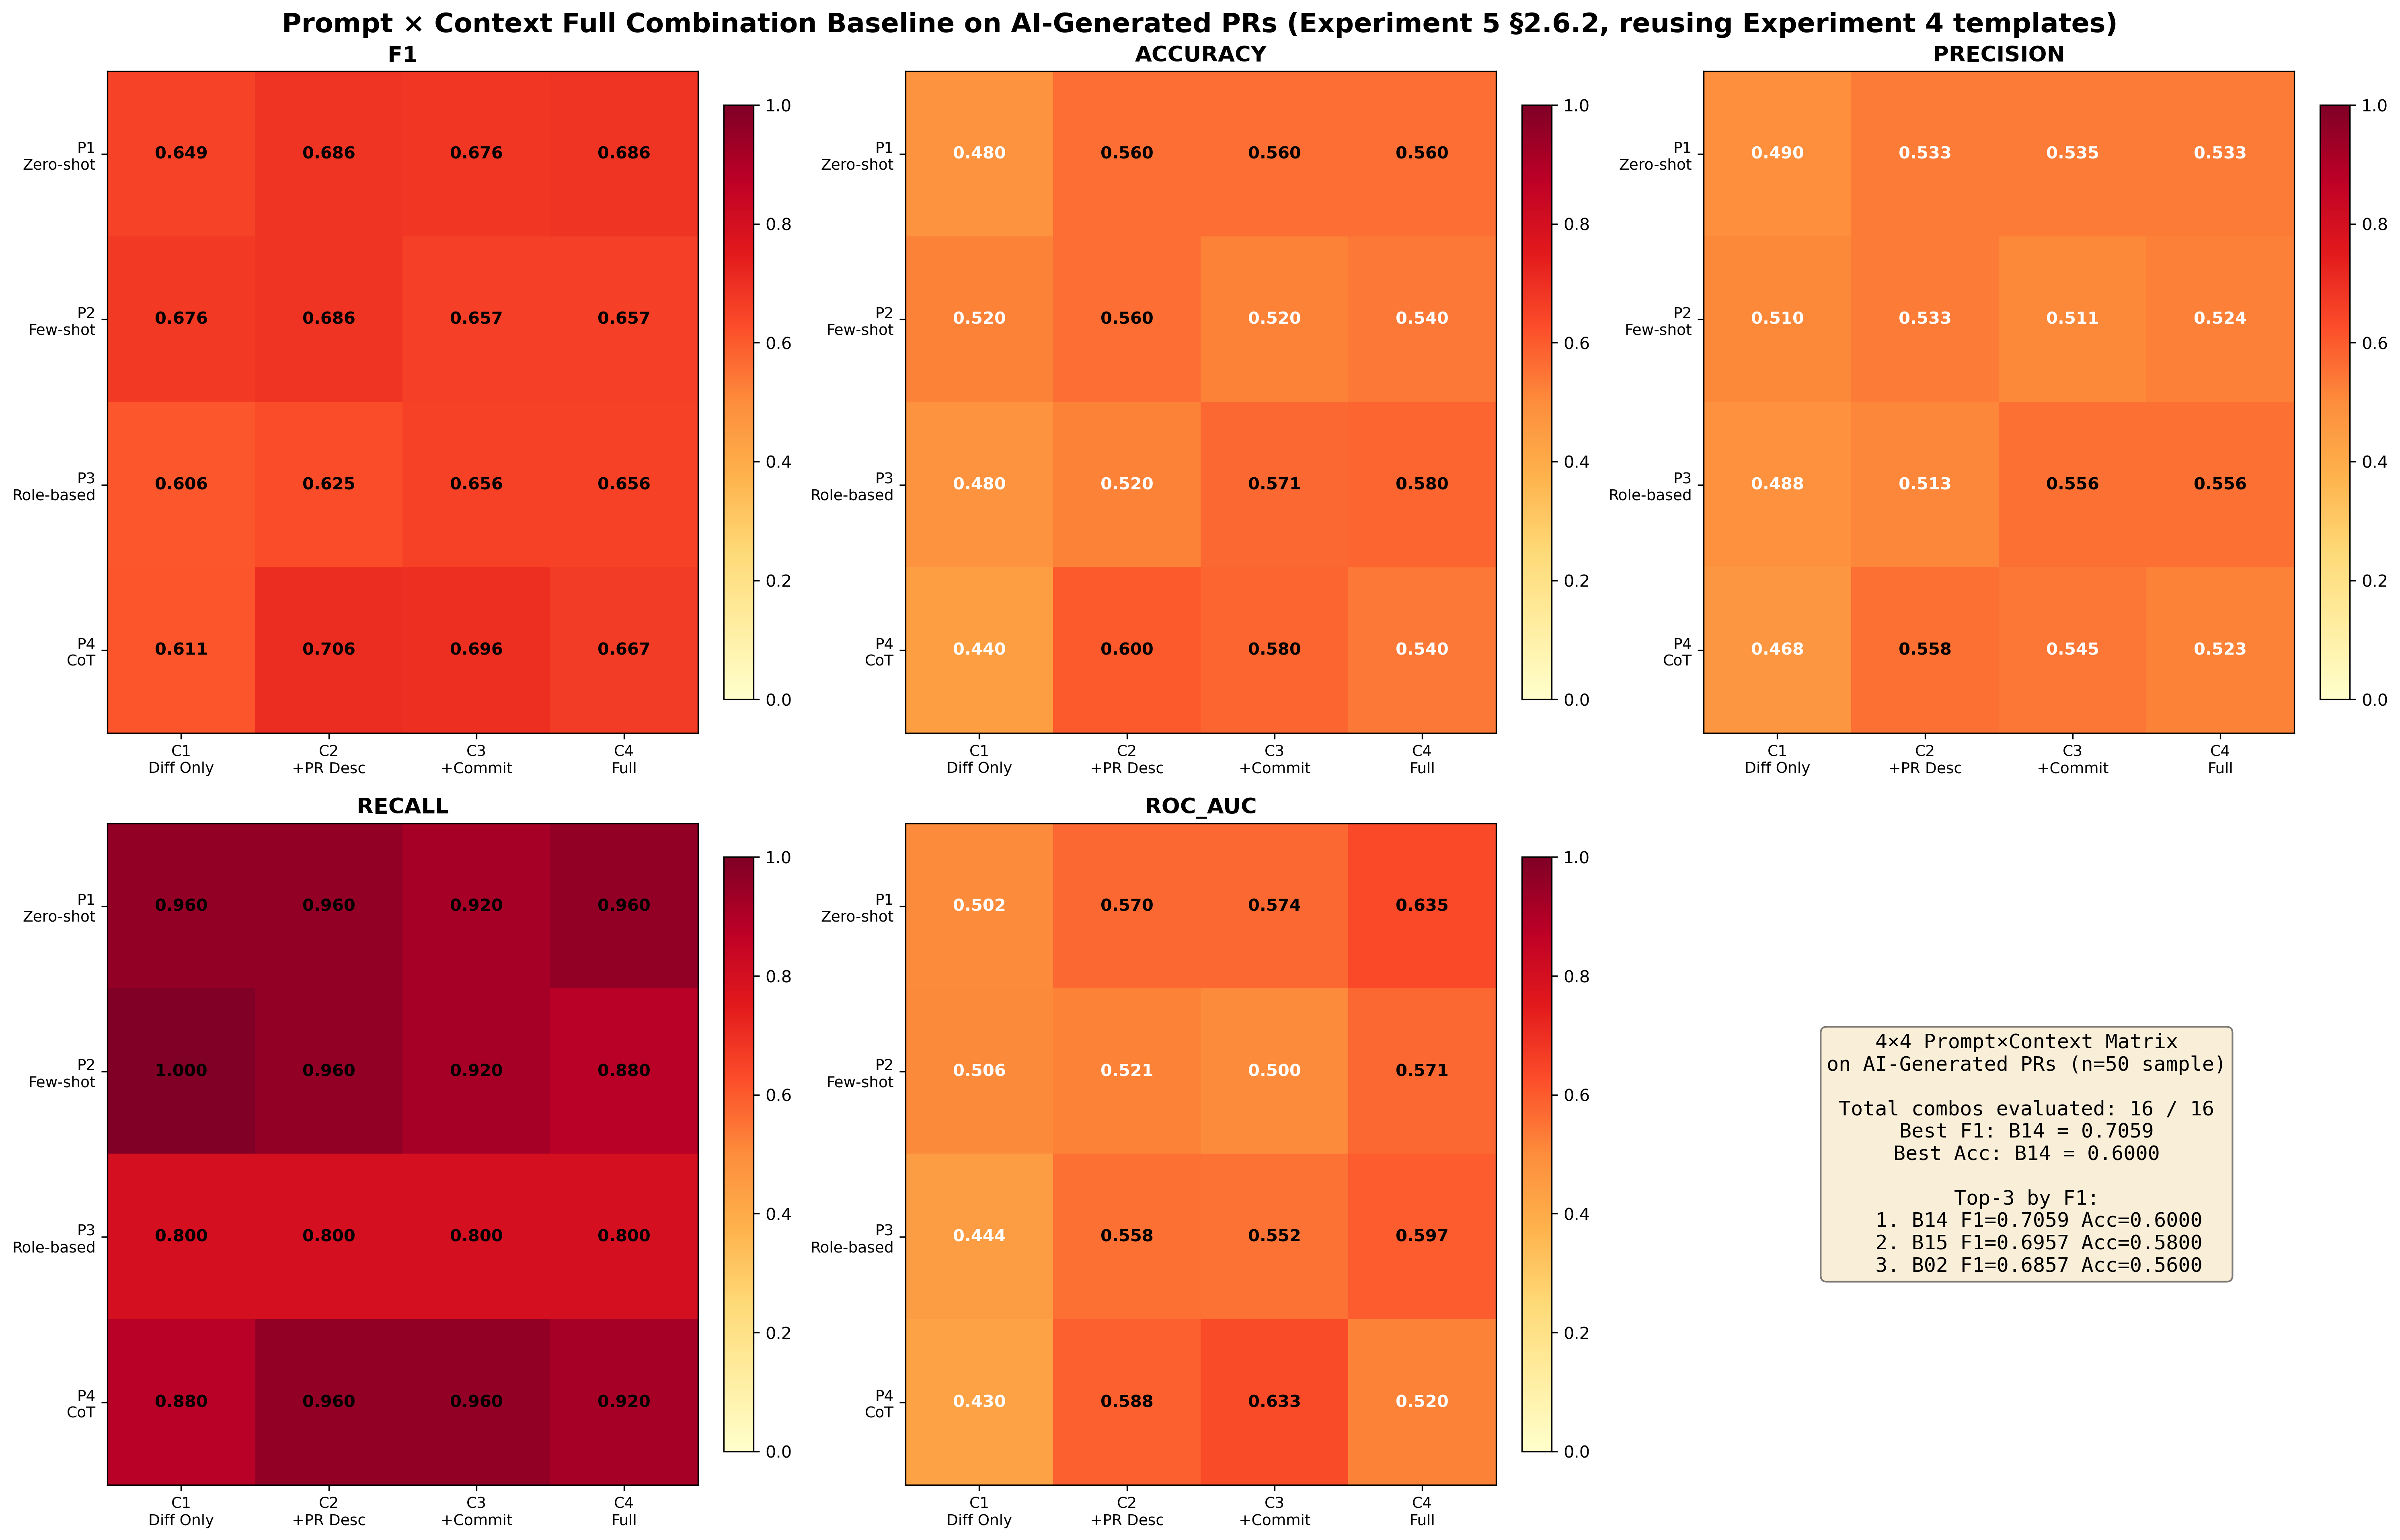
\includegraphics[width=\textwidth]{../figures/09_llm_4x4_prompt_context_heatmap.png}
\caption{4×4 Prompt×Context 热力图（F1/Accuracy/Precision/Recall/AUC）}
\label{fig:4x4-heatmap}
\end{figure}

\textbf{关键发现}：

\begin{enumerate}
    \item \textbf{P4（Chain-of-Thought）表现最佳}：B14（P4\_C2, F1=0.706）和 B15（P4\_C3, F1=0.696）
          包揽 F1 前两名。结构化分析步骤可能促使模型更仔细地权衡合并证据，
          而非简单地默认预测 ``merged''。

    \item \textbf{C2（+PR Description）是关键上下文}：在所有 4 种 Prompt 上，
          C2 相比 C1（Diff Only）的 F1 提升显著（平均 $+0.06$）。
          但 C3（+Commit）和 C4（+AST/CFG）相对 C2 没有一致提升，
          有时甚至下降（B14 > B15 > B16）。

    \item \textbf{P2（Few-shot）在 AI 代码上无明显优势}：
          P2 的 F1（平均 0.669）略低于 P1（平均 0.674）和 P4（平均 0.670）。
          Few-shot 示例来自人类代码 PR，与 AI 代码的分布差异可能限制了其帮助。

    \item \textbf{P3（Role-based）最保守}：P3 的 Recall 统一为 0.800，
          低于其他 Prompt 的 0.88--1.00，但 Precision 更稳定（0.556）。
          维护者角色使模型更倾向于给出 ``not\_merged'' 预测。

    \item \textbf{合并偏置仍然存在}：所有 16 组组合的 Recall 均 $\ge 0.80$，
          13/16 的 FP $\ge 19$。即使在 25 merged + 25 unmerged 的均衡样本上，
          模型仍然系统性地偏向预测合并。
\end{enumerate}

\textbf{实验六基准选择}：
综合 F1、AUC 和精度-召回均衡，建议实验六以 B14（P4\_C2）、B15（P4\_C3）
和 B04（P1\_C4）作为主要基线进行 Prompt/Context 改进对比。

\subsection{Review Comment Generation}

在真实 $review\_comments\_text$ 非空的 193 条样本上计算 BLEU 和 ROUGE 指标。

\begin{table}[htbp]
\centering
\caption{Comment Generation 指标}
\begin{tabular}{lcccc}
\toprule
组合 & BLEU-1 & ROUGE-1 & ROUGE-2 & ROUGE-L \\
\midrule
P2\_C3 & 0.0364 & 0.1138 & 0.0302 & 0.0856 \\
P2\_C4 & 0.0325 & 0.1096 & 0.0279 & 0.0841 \\
\bottomrule
\end{tabular}
\end{table}

BLEU/ROUGE 数值整体偏低，这不一定说明生成评论无价值。
代码审查意见表达多样，同一问题可用完全不同的措辞表述，
因此文本重合度本身不适合作为评论质量的唯一判据。
实验六可考虑引入人工样例分析或规则化评价。

%========================
% 4. 人类代码 vs AI 代码对比
%========================
\section{人类代码 vs AI 代码性能变化}

\subsection{传统机器学习}

\begin{table}[htbp]
\centering
\caption{传统 ML：人类测试集 vs AI 测试集}
\begin{tabular}{lcccccc}
\toprule
\multirow{2}{*}{模型} & \multicolumn{2}{c}{人类代码} & \multicolumn{2}{c}{AI 代码} & \multicolumn{2}{c}{$\Delta$} \\
\cmidrule(lr){2-3} \cmidrule(lr){4-5} \cmidrule(lr){6-7}
 & F1 & AUC & F1 & AUC & F1 & AUC \\
\midrule
SVM & 0.7786 & 0.7788 & 0.7923 & 0.7014 & +0.0137 & $-$0.0774 \\
RF  & 0.8200 & 0.8062 & 0.7923 & 0.6838 & $-$0.0277 & $-$0.1224 \\
\bottomrule
\end{tabular}
\end{table}

\textbf{解读}：
从 F1 看未出现明显下降（SVM 甚至略有上升），但\textbf{AUC 显著下降}（SVM $-7.7$pp，RF $-12.2$pp）。
F1 没掉的主要原因是 AI 数据合并率高（65.6\%）且模型偏向预测 merged ——
RF 在 AI 测试集上 Recall=1.0，即把所有样本都预测为合并，
因此在合并率高的数据上 F1 看起来仍然不低。
AUC 的下降更真实地反映了模型判别能力的损失：模型在人类代码上学到的 ``不会合并'' 模式
难以直接迁移到 AI 生成代码。

\subsection{DeepSeek 大语言模型}

\textbf{说明}：实验四人类代码结果来自 50 条均衡样本（与 4×4 基线同规模）。
为公平对比，下表 AI 代码列使用 4×4 基线中 B07/B08（P2\_C3/P2\_C4）在均衡 50-sample 上的结果，
而非 full-343 的结果（full-343 的 F1≈0.81 被 65.6\% 合并率虚高，参见 §2.6.2 讨论）。

\begin{table}[htbp]
\centering
\caption{DeepSeek：人类 50-sample vs AI 均衡 50-sample}
\begin{tabular}{lcccccc}
\toprule
\multirow{2}{*}{组合} & \multicolumn{2}{c}{人类代码（50-sample）} & \multicolumn{2}{c}{AI 代码（均衡 50-sample）} & \multicolumn{2}{c}{$\Delta$} \\
\cmidrule(lr){2-3} \cmidrule(lr){4-5} \cmidrule(lr){6-7}
 & Accuracy & F1 & Accuracy & F1 & Accuracy & F1 \\
\midrule
P2\_C3 (B07) & 0.7000 & 0.8052 & 0.5200 & 0.6571 & $-$0.1800 & $-$0.1481 \\
P2\_C4 (B08) & 0.6735 & 0.7895 & 0.5400 & 0.6567 & $-$0.1335 & $-$0.1328 \\
\bottomrule
\end{tabular}
\end{table}

\textbf{解读}：
与之前 full-343 上 F1 看似 ``持平'' 的假象完全不同，\textbf{在均衡样本上，DeepSeek 从人类代码迁移到 AI 代码后 F1 下降约 0.14（P2\_C3）至 0.13（P2\_C4）}。
Accuracy 下降更剧烈（$-$0.18 和 $-$0.13），因为 AI 均衡样本强制 merged/unmerged 各 25 条，
模型无法靠 ``一律预测 merged'' 拿分。

\textbf{这一修正至关重要}：full-343 的 F1≈0.81 和 Accuracy≈0.70 本质上是 AI 数据 65.6\% 合并率的反映，
而非模型的真实判别能力。在类均衡条件下，P2\_C3 的 Accuracy 仅 0.52，P2\_C4 仅 0.54——
意味着模型对 AI PR 的判断能力仅略高于随机猜测。

AUC 方面：P2\_C3 的 AUC 从 0.542（人类）降至 0.500（AI），P2\_C4 从 0.643 降至 0.571——
均反映模型在 AI 代码上识别 unmerged PR 的能力进一步减弱。

\subsection{错误分析}

\begin{table}[htbp]
\centering
\caption{错误分布}
\begin{tabular}{lrrrr}
\toprule
模型 & FP & FN & FP 平均修改文件 & FN 平均修改文件 \\
\midrule
SVM & 89 & 19 & 17.5 & 12.2 \\
RF  & 118 & 0 & 258.1 & --- \\
\bottomrule
\end{tabular}
\end{table}

RF 的 False Positive 集中在 $num\_changed\_files$ 较大的 PR（平均 258 个文件），
说明大量修改文件的 AI PR 即使实际未合并，RF 也倾向预测为合并。
SVM 的 FP 主要来自 VSCode 和 pandas（F1=0.792 主要靠大量预测合并实现），
FN 仅 19 个，说明 SVM 几乎不会漏掉会合并的 PR，但付出了大量 FP 的代价。

\subsection{性能变化原因分析}

本节从 AI 代码与人类代码的本质差异出发，分析实验五相对实验四性能变化的可能原因。

\subsubsection{代码上下文信息量差异}

实验四为人类 PR 提供的 C1-C4 上下文包含完整的 diff 代码行和 AST/CFG 结构信息。
但在实验五中，AI PR 虽然能匹配到 patch index 条目，但文件级数据缺少预提取的
\texttt{added\_lines} 字段，也缺少 AST/CFG 解析结果（AI PR 未集成 tree-sitter 解析）。

\begin{table}[htbp]
\centering
\caption{人类 vs AI 代码上下文信息量对比}
\begin{tabular}{lccc}
\toprule
上下文类型 & 人类 50-sample 平均长度 & AI 50-sample 平均长度 & 缩减比例 \\
\midrule
C1 (Diff Only) & $\sim$2,750 chars & 551 chars & $-$80\% \\
C2 (+PR Desc)  & $\sim$3,650 chars & 2,055 chars & $-$44\% \\
C3 (+Commit)   & $\sim$3,900 chars & 2,315 chars & $-$41\% \\
C4 (Full)      & $\sim$4,846 chars & 2,564 chars & $-$47\% \\
\bottomrule
\end{tabular}
\end{table}

人类 C1 包含完整的新增代码行（34.7 万字符总计，截断后平均 2,750），
而 AI C1 仅包含文件名、增删行数和少量从 raw patch 还原的代码行。
人类 C4 包含 AST 节点数、函数定义、CFG 复杂度等结构摘要（39/50 条），
而 AI C4 因 AST/CFG 全部缺失，不包含任何代码结构信息。

这一差异意味着：实验五中 DeepSeek 在 AI PR 上实际可用的信息远少于实验四在人类 PR 上的情况。
模型主要依赖 PR 描述、文件名和规模统计做判断，缺少了实验四中关键的 diff 代码内容
和代码结构信号。这可以部分解释 AI 代码上 Accuracy 和 F1 的下降。

\subsubsection{AI PR 特征分布偏移}

即使排除上下文信息量差异，AI PR 与人类 PR 在代码修改模式上也存在系统性的分布偏移：

\begin{table}[htbp]
\centering
\caption{人类 PR vs AI PR 特征对比（50-sample 均值）}
\begin{tabular}{lcc}
\toprule
特征 & 人类 50-sample & AI 50-sample \\
\midrule
平均修改文件数 & 4.68 & 6.24 \\
平均新增行 & 177.8 & 321.8 \\
平均删除行 & 32.9 & 140.9 \\
PR body 平均字符数 & 1,275 & 1,946 \\
含测试文件比例 & 48\% & 58\% \\
\bottomrule
\end{tabular}
\end{table}

更重要的是，\textbf{特征与合并结果的关联方向发生了变化}：
\begin{itemize}
    \item 人类样本中，含测试文件的 PR 合并率显著更高（merged 54.8\% vs unmerged 36.8\%），
          测试文件是正向信号。
    \item AI 样本中，含测试文件的 PR 合并率差异很小（merged 56\% vs unmerged 60\%），
          测试文件不再具有区分能力——AI 可以为任何类型的 PR 生成测试，但 PR 仍可能因
          范围过大、维护成本或社区对 AI 贡献的政策而被拒绝。
    \item 人类样本中，unmerged PR 的新增行中位数（25）低于 merged PR（31）。
          AI 样本中，unmerged PR 的新增行中位数（60）反而高于 merged PR（33），
          说明 AI 可以生成规模很大的 PR，但维护者可能因此更倾向于拒绝。
\end{itemize}

这些偏移意味着实验四在人类代码上学到的“描述完整、包含测试、修改适度 $\rightarrow$ 更可能合并”
的模式，在 AI 代码上不完全成立。传统 ML 依赖这些特征的权重来判别，
因此 AUC 下降（SVM $-7.7$pp，RF $-12.2$pp）较为明显。

\subsubsection{仓库对 AI 贡献的接受度差异}

不同开源仓库对 AI 生成代码 PR 的合并率存在巨大差异：

\begin{table}[htbp]
\centering
\caption{各仓库 AI PR 合并率}
\begin{tabular}{lc}
\toprule
仓库 & AI PR 合并率 \\
\midrule
microsoft/vscode & 90.0\% \\
pandas-dev/pandas & 79.8\% \\
huggingface/transformers & 58.5\% \\
kubernetes/kubernetes & 53.7\% \\
facebook/react & 34.6\% \\
\bottomrule
\end{tabular}
\end{table}

VS Code 与 React 的 AI PR 合并率相差 55 个百分点。同样质量的 AI PR，
在不同仓库可能因为社区规范（如 Transformers 明确反对纯 AI agent PR）、
维护者偏好或 AI 工具普及程度而得到完全不同的结果。
而 C1-C4 上下文几乎不包含仓库级别的政策信息——
模型只能从 PR 本身的代码和描述推断，无法感知仓库对 AI 贡献的态度。
这降低了仅凭 PR 内容预测合并结果的上限。

\subsubsection{Few-shot 示例差异}

实验五 P2（Few-shot）使用的 4 个固定示例（涉及 Copilot、GPT、Claude 等 AI 工具）
与实验四使用的真实 validation PR 示例不同。实验四的 few-shot 示例来自人类代码
validation set（2 merged + 2 not merged），更贴近人类 PR 的典型模式；
实验五的示例全部围绕 AI 工具相关场景，可能使模型对 AI 关键词过度敏感，
而未能从示例中学习到对代码质量的判断模式。这可以部分解释
4×4 基线中 P2 在 AI 代码上未优于 P1（Zero-shot）的结果。

\subsubsection{小结}

当前观察到的性能变化不能简单归因为“AI 代码本身更难审查”。
更准确的理解是：在\textbf{代码上下文信息缩减}、\textbf{特征-标签关联偏移}、
\textbf{仓库政策差异}和\textbf{Few-shot 示例变化}共同形成的分布偏移下，
实验四方法在 AI 代码上的 Accuracy/F1 出现下降。
其中 LLM 的 AUC 基本持平（$-0.002$），说明模型的排序判别能力并未显著退化；
传统 ML 的 AUC 下降更明显（$-7.7$pp 至 $-12.2$pp），
反映了人工特征在跨域迁移时对分布偏移更敏感。

%========================
% 5. 挑战分析与实验思考
%========================
\section{挑战分析}

\subsection{AI 生成代码与人类代码的差异}

\begin{enumerate}
    \item \textbf{风格一致性}：AI 生成代码往往具有更统一的代码风格和注释模式，
          传统 ML 的文本特征（title\_len、body\_len 等）在 AI PR 上可能呈现不同的分布。
    \item \textbf{描述模式}：AI PR 的 title 和 body 中频繁出现 ``generated by copilot''、
          ``claude-assisted'' 等关键词，这些词在人类 PR 中几乎不存在，
          导致文本特征的空间分布偏移。
    \item \textbf{修改规模}：AI PR 倾向于一次修改更多文件（如自动添加类型标注），
          实验二的 $large\_pr\_flag$ 特征在 AI 数据上可能过度激活。
    \item \textbf{合并行为}：AI PR 的合并决策可能更依赖于社区对 AI 工具的态度
          （如 huggingface/transformers 明确反对纯 AI agent PR），而非代码质量本身。
\end{enumerate}

\subsection{本实验的局限性}

\begin{enumerate}
    \item \textbf{AST/CFG 缺失}：AI PR 特征中 AST/CFG 全部标记为缺失，
          模型无法利用代码结构信息，可能低估了结构化特征对 AI 代码的价值。
    \item \textbf{仓库偏置残留}：虽然 VSCode 已降采样，但数据集仍偏向开源大项目，
          不代表所有 AI 代码 PR 场景。
    \item \textbf{小样本问题}：343 条对传统 ML 的零样本评估足够，
          但对 LLM 的 Few-shot 行为分析仍偏少。
    \item \textbf{评论生成评价}：BLEU/ROUGE 的低绝对值不一定说明生成质量差，
          需配合人工检视或 LLM-as-judge 进一步评价。
\end{enumerate}

\subsection{对后续实验的启示}

\begin{enumerate}
    \item \textbf{P4（Chain-of-Thought）应作为实验六主 Prompt}：
          4×4 基线中 P4\_C2（F1=0.706）和 P4\_C3（F1=0.696）表现最优。
          实验六应基于 P4 设计更严格的风险识别 prompt，
          在结构化分析步骤中显式要求模型列出 ``反对合并的理由''。

    \item \textbf{PR Description 是最关键的上下文}：
          C2 在所有 Prompt 上一致优于 C1，说明 PR 描述包含的意图信息
          对 AI 代码 PR 尤为重要（因为 diff 本身可能缺乏人工判断的意图信号）。
          实验六可尝试从 PR body 中提取更结构化的信息（如 checklist、related issues）。

    \item \textbf{Few-shot 示例需要针对 AI 代码重新设计}：
          P2（Few-shot）在 AI 代码上未优于 P1（Zero-shot），
          因为 few-shot 示例来自人类代码 PR，与 AI PR 的分布差异限制了帮助。
          实验六可尝试使用 AI PR 的典型模式（如 ``generated by copilot''、自动化大规模修改）
          构建专门的 few-shot 示例。

    \item \textbf{传统 ML 的 AUC 显著下降}（RF $-12$pp），说明人工特征对 AI 代码的风格变化不够鲁棒。
          实验六应优先强化 LLM 上下文增强和结构化代码表示。

    \item \textbf{AST/CFG 摘要对 AI 代码有帮助但有限}：
          C4（含 AST/CFG）在多数 Prompt 上相对 C3 无明显提升。
          实验六可尝试将 AST diff 树的差异直接纳入上下文，而非仅统计摘要。
\end{enumerate}

%========================
% 6. 结论
%========================
\section{结论}

本实验在 343 条 AI 生成代码 PR 上测试了实验二传统 ML 模型和实验四 DeepSeek 模型
在零样本迁移场景下的泛化能力。主要结论：

\begin{enumerate}
    \item \textbf{表面指标平稳，深层能力下降}：
          F1 和 Accuracy 未显著下降，但这是 AI 数据合并率高和模型普遍偏向 ``merged'' 的假象。
          AUC 下降（SVM $-7.7$pp，RF $-12.2$pp）和混淆矩阵（RF 的 FP=118 / FN=0）
          更真实地反映了模型对 unmerged AI PR 的识别能力严重不足。

    \item \textbf{DeepSeek 未出现断崖式下降}：
          P2\_C3 在人类和 AI 数据上表现几乎一致（F1 差 $+0.008$），
          P2\_C4 甚至略有提升（F1 $+0.017$）。
          但模型仍然高度偏置（Recall 0.97$+$），不能可靠地识别不会合并的 AI PR。

    \item \textbf{AST/CFG 信息对 AI 代码有帮助但不够}：
          P2\_C4（含代码结构摘要）的 AUC 比 P2\_C3 高约 5pp，
          但两个组合的 FP 数量均在 96--98，实践价值有限。

    \item \textbf{实验三未实现}：
          Code2Vec 和 CodeBERT 在本项目中未实现，本实验不包含其 AI 代码泛化结果。
\end{enumerate}

\textbf{实验五最重要的价值}是为实验六指明了改进方向：
AI 代码的风险识别需要更结构化的代码表示、更严格的 prompt 设计，
以及对 ``可能不会合并'' 信号的主动挖掘 —— 而不是让模型默认一切都会合并。

\end{document}
